\documentclass[a4paper,twocolumn]{oblivoir}
\usepackage{amsmath,amssymb,kotex,kswrapfig,mdframed,paralist,graphicx}
\usepackage{fapapersize}
%\usefapapersize{210mm,297mm,10mm,*,10mm,*}

\usepackage{tabto,pifont}
\TabPositions{0.2\textwidth,0.4\textwidth,0.6\textwidth,0.8\textwidth}
\newcommand\tabb[5]{\par\noindent
\ding{172}\:{\ensuremath{#1}}
\tab\ding{173}\:\:{\ensuremath{#2}}
\tab\ding{174}\:\:{\ensuremath{#3}}
\tab\ding{175}\:\:{\ensuremath{#4}}
\tab\ding{176}\:\:{\ensuremath{#5}}}

\newcommand\tabc[5]{\par\bigskip\noindent
\ding{172}\:{\ensuremath{#1}}
\tabto{0.25\textwidth}\ding{173}\:\:{\ensuremath{#2}}\medskip\par\noindent
\ding{174}\:\:{\ensuremath{#3}}
\tabto{0.25\textwidth}\ding{175}\:\:{\ensuremath{#4}}\medskip\par\noindent
\ding{176}\:\:{\ensuremath{#5}}}

\newcommand\tabd[5]{\par\bigskip\noindent
\ding{172}\:{#1}\medskip\par\noindent
\ding{173}\:\:{#2}\medskip\par\noindent
\ding{174}\:\:{#3}\medskip\par\noindent
\ding{175}\:\:{#4}\medskip\par\noindent
\ding{176}\:\:{#5}}


%\pagestyle{empty}

%%% Counters
\newcounter{num}
\newcounter{answer}

%%% Commands
\newcommand\prob[1]
{\vs\par\noindent\stepcounter{num} \textbf{문제 \thenum) #1}\par\noindent}

\newcommand\exam[1]
{\vs\par\noindent\stepcounter{num} \textbf{예제 \thenum) #1}\par\noindent}

\newenvironment{expl}{\begin{mdframed}[frametitle=풀이]}{\end{mdframed}}

\newcommand\pb[1]{\ensuremath{\fbox{\phantom{#1}}}}

\newcommand\vs[1]{\vspace{30pt}}

\newcommand\an{\bigskip\par\noindent\stepcounter{answer}\textbf{문제 \theanswer)}\par\noindent}

%%% Meta Commands
%\let\oldsection\section
%\renewcommand\section{\clearpage\oldsection}

\let\emph\textsf

\begin{document}
\title{태희 : 3-1 중간고사 대비 문제}
\date{\today}
\author{}
\maketitle

%%
\section{절댓값 문제들}

%
\exam{}
\(a>0,\quad b<0\)일 때, \(\sqrt{a^2}+\sqrt{4b^2}\)을 간단히 하여라.
\begin{expl}
\begin{align*}
\sqrt{a^2}+\sqrt{4b^2}
&=\sqrt{a^2}+\sqrt{(2b)^2}\\
&=|a|+|2b|\\
&=a+(-2b)=a-2b
\end{align*}
\end{expl}

%
\prob{}
\(a<0,\quad b>0\)일 때, \(\sqrt{4a^2}+\sqrt{9b^2}\)을 간단히 하여라.
\tabc{2a+3b}{2a-3b}{-2a+3b}{-2a-3b}{a+b}
\newpage

%
\exam{개념+유형, 개념편 p26 \#8}
\(a>0,\quad ab<0\)일 때, \(\sqrt{(-a)^2}+\sqrt{9a^2}-\sqrt{4b^2}\)을 간단히 하여라.
\begin{expl}
\(a>0\)이고 \(b<0\)이다.
따라서
\begin{align*}
&\sqrt{(-a)^2}+\sqrt{9a^2}-\sqrt{4b^2}\\
=&|-a|+|3a|-|2b|\\
=&-(-a)+(3a)-(-2b)=4a+2b
\end{align*}
\end{expl}

%
\prob{개념+유형, 유형편 p8 \#20}
\(a>b,\quad ab<0\)일 때, \((-\sqrt{a})^2-\sqrt{(-a)^2}+\sqrt{9b^2}\)을 간단히 하면?
\tabb{a+b}{a-3b}{b}{-3b}{3b}

\newpage
%
\exam{개념+유형, 개념편 p28 \#28}
\(0<a<1\)일 때,
\[\displaystyle\sqrt{\left(a+\frac1a\right)^2}-\sqrt{\left(a-\frac1a\right)^2}-\sqrt{(2a)^2}\]
을 간단히 하여라.
\begin{expl}
\(a>0\)이므로
\[a+\frac1a>0\]
\(0<a<1\)이므로 \(\frac1a>1\)이고, 따라서\(\frac1a>a\).
그러므로
\[a-\frac1a<0\]
또한
\[2a>0\]
그러므로
\begin{align*}
&\sqrt{\left(a+\frac1a\right)^2}-\sqrt{\left(a-\frac1a\right)^2}-\sqrt{(2a)^2}\\[10pt]
=&\left|a+\frac1a\right|-\left|a-\frac1a\right|-|2a|\\[10pt]
=&\left(a+\frac1a\right)-\left\{-\left(a-\frac1a\right)\right\}-2a\\[10pt]
=&\left(a+\frac1a\right)+\left(a-\frac1a\right)-2a\\[10pt]
=&0
\end{align*}
\end{expl}

%
\prob{}
\(0<a<1\)일 때,\\
\(\displaystyle\sqrt{\left(\frac1a+a\right)^2}+\sqrt{\left(\frac1a-a\right)^2}\)을 간단히 하여라.
\par\bigskip
\tabb{2a}a0{\frac1a}{\frac2a}


%
\prob{}
\(a>1\)일 때,\\
\(\displaystyle\sqrt{a^2}-\sqrt{\left(a-\frac1a\right)^2}\)\를 간단히 하여라.

%%
\exam{개념+유형, 유형편 p21 \#21}
\(a<0<b<1\)일 때,
\begin{multline*}
\sqrt{(a-b)^2}+\sqrt{\left(b-\frac1b\right)^2}\\
-\sqrt{\left(b+\frac1b\right)^2}-\sqrt{(-a)^2}
\end{multline*}
을 간단히 하여라.
\begin{expl}
\(a<b\)로부터
\[a-b<0\]
\(0<b<1\)로부터 \(\frac1b>1\).
따라서 \(b<\frac1b\).
그러므로
\[b-\frac1b<0\]
\(b>0\)으로부터
\[b+\frac1b>0\]
\(a<0\)으로부터
\[-a>0\]
따라서
\begin{align*}
&(준식)\\
=&|a-b|+\left|b-\frac1b\right|-\left|b+\frac1b\right|-|-a|\\
=&-(a-b)-\left(b-\frac1b\right)-\left(b+\frac1b\right)-(-a)\\
=&-a+b-b+\frac1b-b-\frac1b+a=-b
\end{align*}
\end{expl}

%
\prob{}
\(a<0<b<1\)일 때,
\[\sqrt{a^2}+\sqrt{\left(\frac1b-b\right)^2}+\sqrt{\left(\frac1b+b\right)^2}\]
을 간단히 하여라.

%
\prob{}
\(0<a<1<b\)일 때,
\[\sqrt{a^2}+\sqrt{(a-b)^2}-\sqrt{\left(b-\frac1b\right)^2}\]
을 간단히 하여라.
\newpage

%%
\section{교과서, 기출}

%
\prob{2017 장위중 기출, \#1}
\(x\)가 \(6\)의 제곱근일 때, 다음 중 \(x\)와 \(6\) 사이의 관계식을 바르게 나타낸 것은?
\tabc
{x^2=6}
{x=6^2}
{\sqrt x=6}
{x=\sqrt6}
{x=-\sqrt6}

%
\prob{p 24}
다음 중 실수 \(a\)가 유리수인 경우를 고르시오.
\tabd
{A4용지의 가로, 세로의 길이의 비는 \(1:\sqrt2\)이다. 이때, \(a=\sqrt2\)}
{황금비는 \(1:\frac{1+\sqrt5}2\)이다. 이때, \(a=\frac{1+\sqrt5}2\)}
{지름의 길이가 1m인 트랙터 바퀴가 한 바퀴 굴러간 거리는 \(\pi\)m이다. 이때 \(a=\pi\)}
{\(a=\sqrt{0.\stackrel{\cdot}4}\)}
{\(a\)는 \(\sqrt 7\)의 소수부분}

%
\prob{p 26}
다음 중 틀린 것을 고르시오.
\tabd
{\(5\)의 제곱근은 \(\sqrt5\)와 \(-\sqrt5\)이다.}
{\(0\)의 제곱근은 1개이다.}
{\(4\)의 음의 제곱근은 \(-2\)이다.}
{제곱근 \(9\)는 \(3\)이다.}
{어떤 수의 제곱근은 항상 무리수이다.}
\newpage

%
\prob{p 26}
다음 식을 계산하시오
\begin{multline*}
\sqrt{1^3+2^3+3^3}+\sqrt{1^3+2^3+3^3+4^3}\\+\sqrt{1^3+2^3+3^3+4^3+5^3}
\end{multline*}
\tabb{27}{28}{29}{30}{31}

%
\prob{p 42}
실수 \(a\), \(b\)에 대하여 다음 중 옳은 것을 고르시오.
\tabd
{\(a\)와 \(b\)가 모두 유리수이면 \(a+b\)는 무리수이다.}
{\(a\)와 \(b\)가 모두 무리수이면 \(a+b\)는 무리수이다.}
{\(a\)와 \(b\)가 모두 무리수이면 \(a\times b\)는 유리수이다.}
{\(a\)가 유리수이고 \(b\)가 무리수이면 \(a+b\)는 무리수이다.}
{\(a\)가 유리수이고 \(b\)가 무리수이면 \(a\times b\)는 무리수이다.}

%
\noindent
\begin{minipage}{0.2\textwidth}
\prob{p 43}
오른쪽 그림과 같은 원뿔대의 부피를 구하여라.
\end{minipage}
%
\begin{minipage}{0.2\textwidth}
\bigskip\bigskip
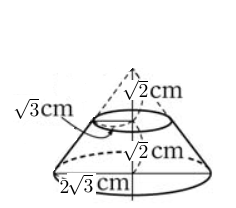
\includegraphics{cone}
\end{minipage}
\par\bigskip
\tabb
{6\sqrt2\pi}
{7\sqrt2\pi}
{8\sqrt2\pi}
{9\sqrt2\pi}
{10\sqrt2\pi}

%
\noindent
\begin{minipage}{0.2\textwidth}
\prob{p 43}
오른쪽 그림과 같은 사각뿔대의 부피를 구하여라.
\end{minipage}
%
\begin{minipage}{0.2\textwidth}
\bigskip\bigskip
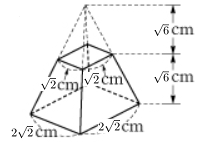
\includegraphics{pyramid}
\end{minipage}
\par\bigskip
\tabb
{\frac{11}3\sqrt6}
{4\sqrt6}
{\frac{13}3\sqrt6}
{\frac{14}3\sqrt6}
{5\sqrt6}

%
\noindent
\begin{minipage}{0.2\textwidth}
\prob{p 44}
오른쪽 그림과 같은 꽃밭의 둘레를 구하여라.
\end{minipage}
%
\begin{minipage}{0.25\textwidth}
\bigskip\bigskip
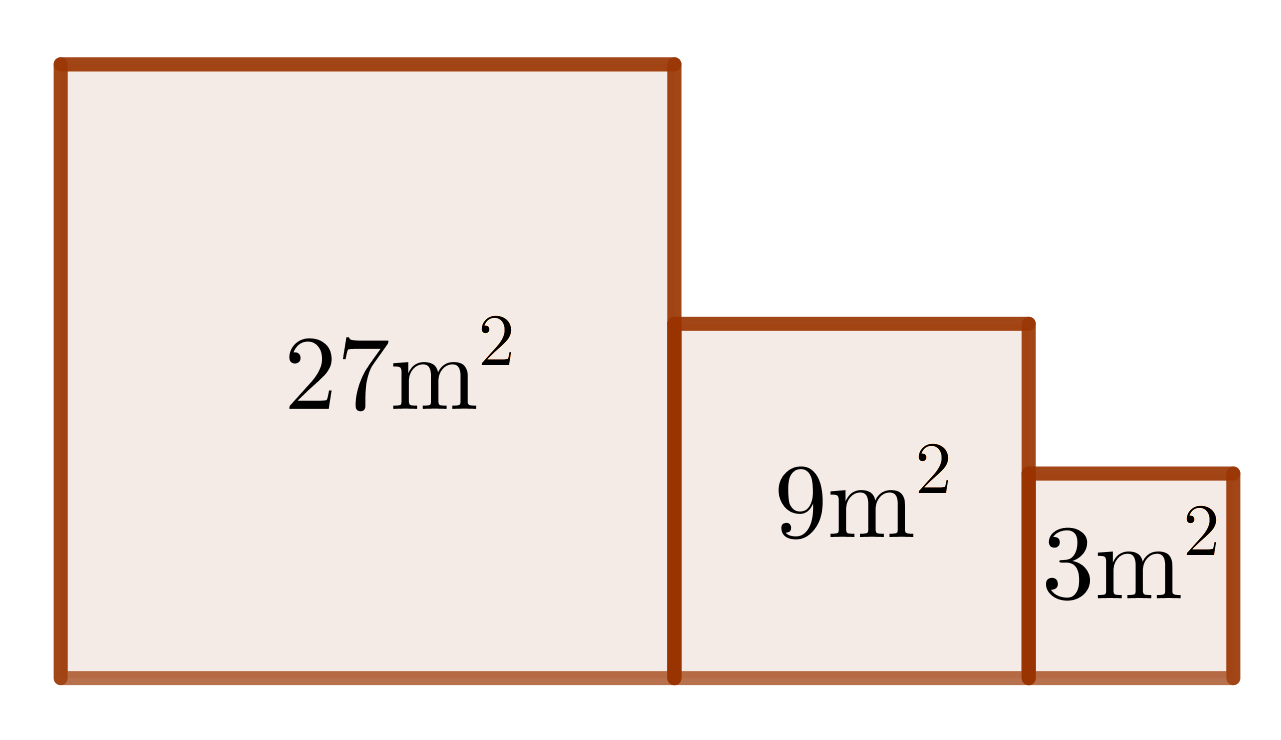
\includegraphics[width=\textwidth]{flowers1}
\end{minipage}
\tabb
{6+14\sqrt3}
{6+15\sqrt3}
{6+16\sqrt3}
{7+14\sqrt3}
{7+15\sqrt3}

%
\noindent
\begin{minipage}{0.2\textwidth}
\prob{p 44}
오른쪽 그림과 같은 꽃밭의 둘레를 구하여라.
\end{minipage}
%
\begin{minipage}{0.25\textwidth}
\bigskip\bigskip
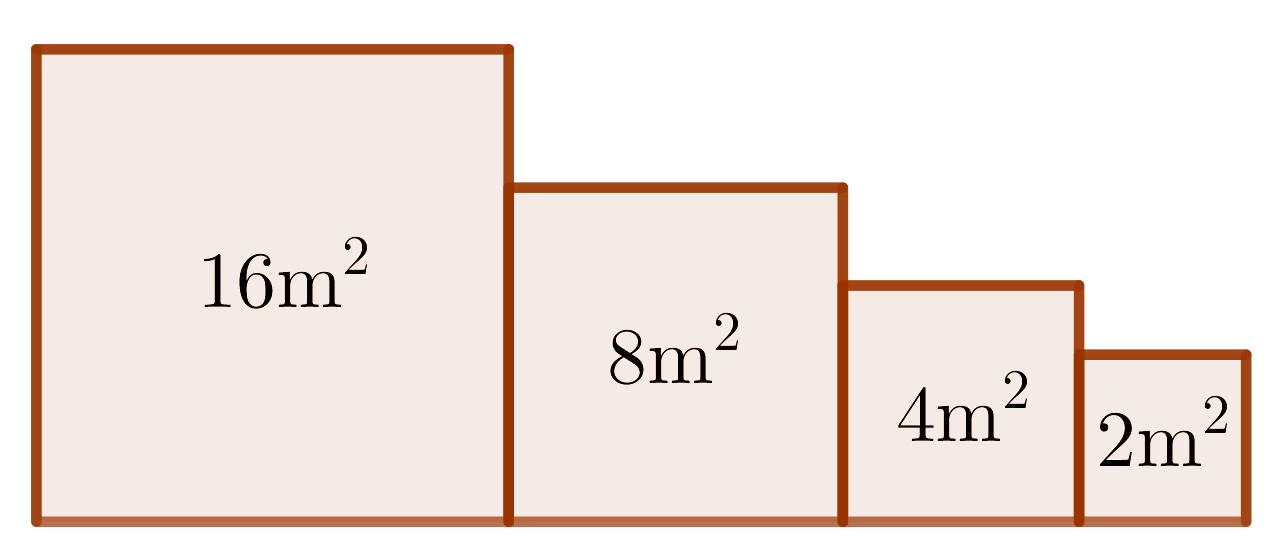
\includegraphics[width=\textwidth]{flowers2}
\end{minipage}
\tabb
{18+4\sqrt2}
{18+6\sqrt2}
{18+8\sqrt2}
{20+4\sqrt2}
{20+6\sqrt2}

%
\noindent
\begin{minipage}{0.2\textwidth}
\prob{p 44}
오른쪽 그림과 같은 꽃밭의 둘레를 구하여라.
\end{minipage}
%
\begin{minipage}{0.25\textwidth}
\bigskip\bigskip
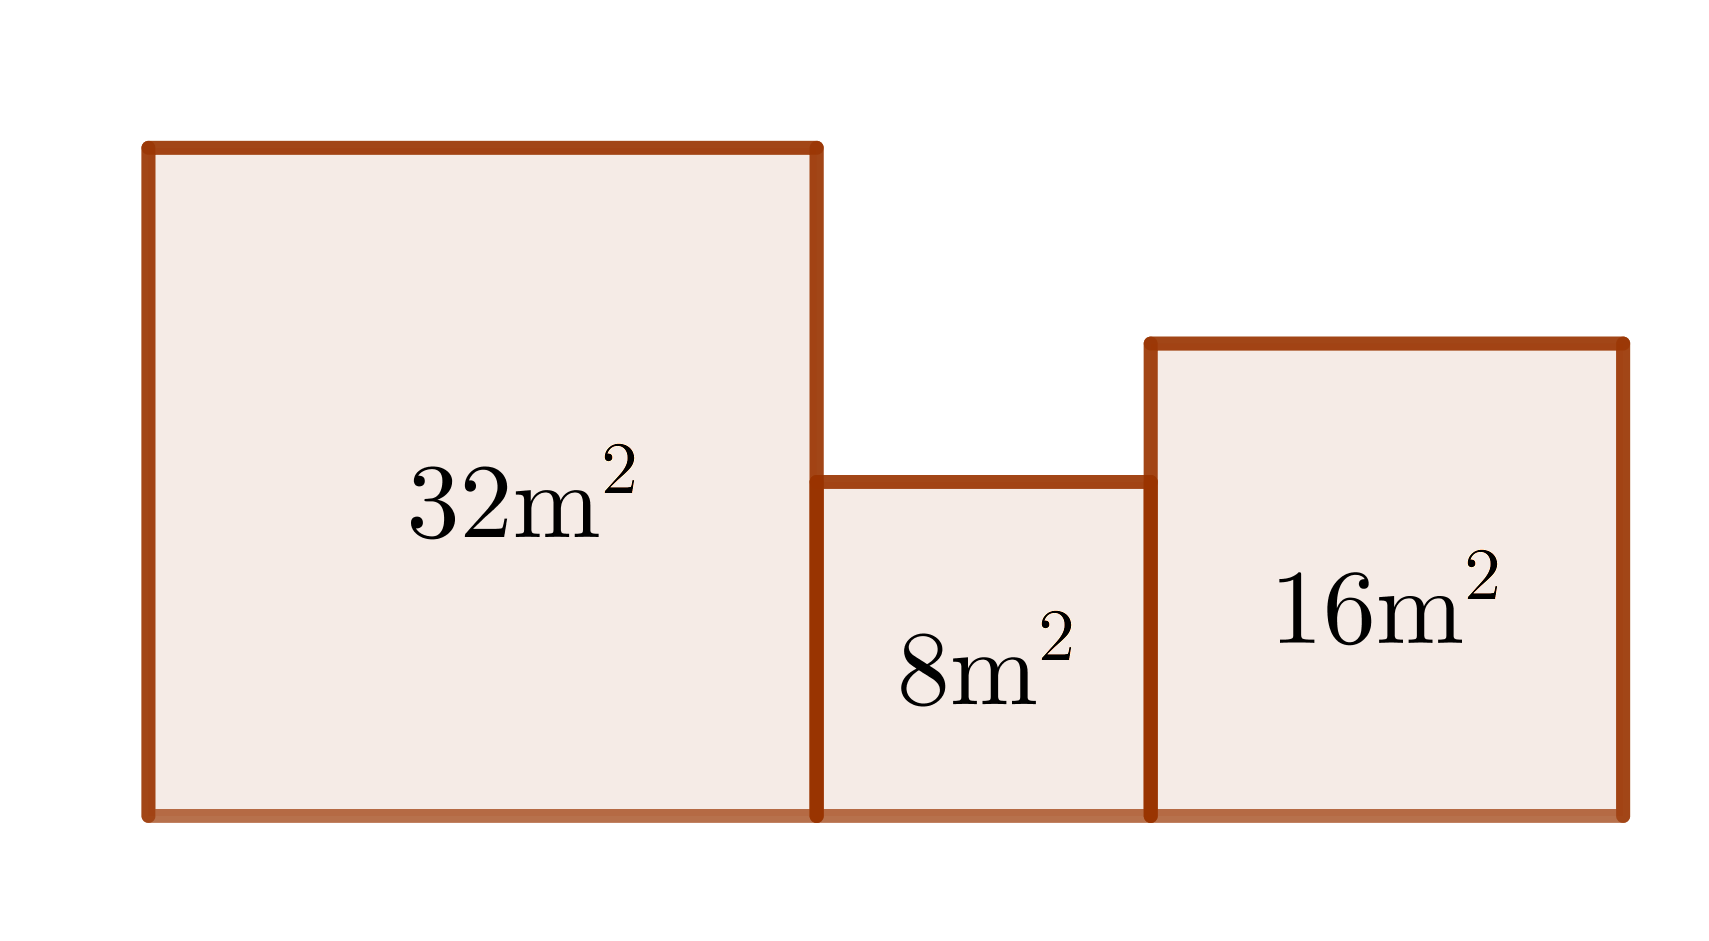
\includegraphics[width=\textwidth]{flowers3}
\end{minipage}
\tabb
{8+8\sqrt2}
{12+12\sqrt2}
{16+16\sqrt2}
{8+12\sqrt2}
{12+16\sqrt2}
\newpage

%
\prob{p 56}
다음 식을 이용하여 아래의 계산을 하여라
\begin{align*}
(10a+5)^2
=&100a^2+100a+25\\
=&100a(a+1)+25
\end{align*}
\begin{enumerate}[(1)]
\item
\(45^2=\)
\item
\(75^2=\)
\item
\(95^2=\)
\end{enumerate}

%
\prob{p 63}
다항식 \(x^2+\pb{10}-6\)이 인수분해가 되도록 하는 정수 \(\pb{10}\)의 값들을 모두 구하여라.
\tabb{-2,-1,1,2}{-3,-1,1,3}{-4,-1,1,4}{-5,-1,1,5}{-6,-1,1,6}

%
\prob{p 63}
다항식 \(2x^2+\pb{10}+3\)이 인수분해가 되도록 하는 정수 \(\pb{10}\)의 값들을 모두 구하여라.
\tabb{-7,-5,5,7}{-7,-4,4,7}{-6,-5,5,6}{-6,-4,4,6}{5,7}

%
\prob{p 65}
인수분해 공식을 이용하여 다음 식의 값을 구하여라.
\[8^2-7^2+6^2-5^2+4^2-3^2+2^2-1^2\]
\tabb{36}{37}{38}{39}{40}
\newpage

%
\exam{p 69}
다음 식에서 자연수 \(n\)의 값을 구하여라.
\[(2+1)(2^2+1)(2^4+1)=2^n-1\]
\begin{expl}
\begin{align*}
&(2+1)(2^2+1)(2^4+1)\\
=&1\times(2+1)(2^2+1)(2^4+1)\\
=&(2-1)(2+1)(2^2+1)(2^4+1)\\
=&(2^2-1)(2^2+1)(2^4+1)\\
=&(2^4-1)(2^4+1)\\
=&2^8-1
\end{align*}
따라서 \(n=8\)
\end{expl}

%
\prob{p 69}
다음 식에서 자연수 \(n\)의 값을 구하여라.
\[(2+1)(2^2+1)=2^n-1\]
\tabb248{16}{32}

%
\prob{p 69}
다음 식에서 자연수 \(n\)의 값을 구하여라.
\[(2+1)(2^2+1)(2^4+1)(2^8+1)=2^n-1\]
\tabb248{16}{32}

%%
\section*{답}

\stepcounter{answer}
%
\an\ding{174}

\stepcounter{answer}
%
\an\ding{175}

\stepcounter{answer}
%
\an\ding{176}

%
\an
\(\frac1a\)

\stepcounter{answer}
%
\an
\(-a+\frac2b\)

%
\an
\(\frac1b\)

%
\an\ding{172}
%
\an\ding{175}

%
\an\ding{176}
%
\an\ding{176}
%
\an\ding{175}
%
\an\ding{173}
%
\an\ding{175}
%
\an\ding{172}
%
\an\ding{176}
%
\an\ding{174}
%
\an
(1) \(2025\), (2) \(5625\), (3) \(9025\)
%
\an\ding{175}
%
\an\ding{172}
%
\an\ding{172}
%
\stepcounter{answer}
%
\an\ding{173}
%
\an\ding{175}

\end{document}